\section{Computational Methods}

Molecular dynamics simulations were all performed using the Amber 11 software suite.\cite{Case2010} Polarizable models for the \wat~and \suldiox~molecules were used in the simulations, and have been used previously in studies on interfacial systems because they are known to more accurately reproduce interfacial structure and free energy profiles.\cite{Wick2007,Rivera2006,Dang1998} The \wat~model used is the POL3 model,\cite{Caldwell1995} and for \suldiox we used the model of Dang, et al. that places a single polarizable center on the sulfur atom.\cite{Baer2010}

All simulations began with an equilibrated cube of 900 \wat~molecules, with sides of length 30\angs. The long axis of each simulation cell (the axis normal to the water surface) was then lengthened to 120\angs, and the systems were further equilibrated for 10 ns. The simulations all employed periodic boundaries to create an ``infinite-slab'' geometry. After equilibrating the neat-\wat~slabs two types of systems were created by introducing \suldiox: a single-\suldiox~system, herein referred to as the ``neat-water'' system, and a saturated \suldiox~system. 

One system involved the addition of a single \suldiox~molecule either within the bulk of the water slab (for equilibrium MD), or above the slab surface (in the SMD simulations). The single-\suldiox~system was then evolved for 2 ns to produce an equilibrated starting configuration. The second system introduced 22 \suldiox~molecules into the water slab in order to saturate it to a level coinciding with the Henry's law constant for \suldiox~in water. Additionally, 50 \suldiox~molecules were introduced into the gas phase outside of the water slab, on both surfaces, to simulate an added 50 atm of \suldiox~gas pressure. The saturated system was then evolved for 2 ns to produce a starting configuration for further saturated simulations.

\subsection{Equilibrium Simulations}

Equilibrium simulations involved adding \suldiox~to a water slab and equilibrating as outlined above. One system had a single \suldiox~added to the center of the water box, representing a concentration of 0.06 M. The complementary saturated system with 22 \suldiox~molecule in the bulk represents a system of concentration 1.35 M, with an additional 50 \suldiox~in the gas phase to model 50 atm of pressure above the water surface. Both the low and high concentration systems were then evolved for a further 10 ns using a timestep of 0.5fs, with atomic coordinates written every 100 fs.

\subsection{Steered Molecular Dynamics Simulations}

% need to add in the specifics about the SMD routine, force constants, calculations, etc.
A second set of simulations involved preparing an equilibrated water slab as in the surface equilibrated method above. However, for both the neat-water and saturated systems, a single \suldiox~was introduced 20\angs above the water slab surface, with the sulfur atom tethered to its initial position. The systems were evolved for 1 ns, taking coordinate snapshots every 20 ps to create 50 starting points for further simulations. Steered molecular dynamics (SMD) were then performed on the 50 system configurations (in both the low and high concentrations) to guide the \suldiox~down towards a tethered water 15\angs under the water slab surface by applying a small steering force.\cite{Isralewitz2001} The \suldiox~thus passed through the continuum of environments from gas phase to (neat- and saturated) water surface adsorption, and finally absorption into the bulk of the \wat~slab. 

Figure \ref{fig:starting-configurations} illustrates two sample starting configurations for the SMD simulations, showing both the neat-\wat~slab and the saturated-\wat~slab configurations before steering the \suldiox~towards the water bulk.

\begin{figure}[h!]
	\begin{center}
		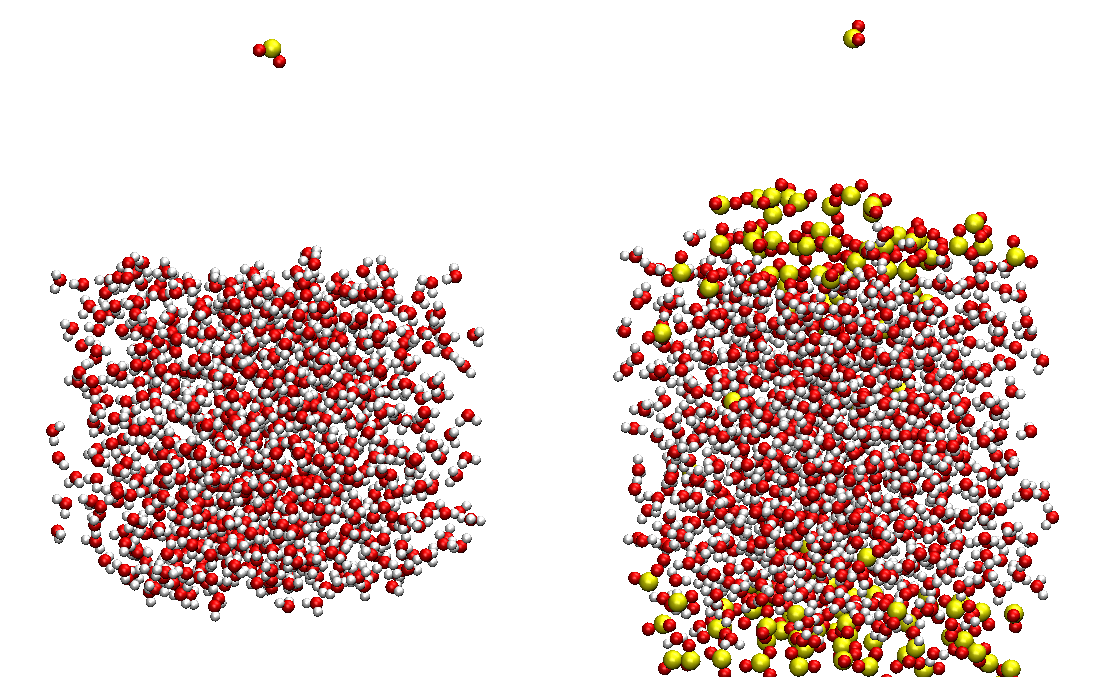
\includegraphics[scale=1.0]{images/startingconfigurations.png}
		\caption{Sample starting configurations for the two types of SMD simulations. The neat-\wat~slab simulation introduces a single \suldiox~molecule that is then guided into the surface of the water and further into the bulk (left). The saturated-\wat~slab simulation begins with different configurations of a water system that has been loaded with \suldiox~to saturate the water phase, and also with a high pressure of \suldiox~gas (right). The single \suldiox~(shown at the top) is then steered through the surface region saturated with \suldiox~molecules, and into the water bulk.}
		\label{fig:starting-configurations}
	\end{center}
\end{figure}
